\documentclass[11pt,a4paper,titlepage]{article}

\usepackage[utf8]{inputenc}
\usepackage[T1]{fontenc}
\usepackage[english]{babel}
\usepackage{color}
\usepackage{graphicx}
\usepackage{amsmath, amssymb}
\usepackage[hmargin={2.5cm,2.5cm},top=2.5cm,bottom=2.5cm]{geometry}
\usepackage[colorlinks=true,breaklinks=true,linkcolor=blue,filecolor=magenta,urlcolor=cyan,pdftitle={IF3E Report},pdfsubject={Martine Travels}]{hyperref}


%opening
\title{IF3E Project Report}
\author{GIRAUX Maxime \and HAUTEFAYE Corentin \and JOURDAN Lorna}
%\date{}

\begin{document}

\maketitle

%-----------------------------------------------
\renewcommand{\abstractname}{Introduction}
\begin{abstract}
	During this part of the semester (\textit{i.e. A24}) we chose to undertake the first subject which was designing a management system for a travel agency. Thus we decided to create a fictive company called \textit{$\sim$Martine Travels\footnote{Copyright \textcopyright Martine Travels 2024}$\sim$} as a reference to those books in which the latter goes to different places such as the beach, mountain, and so on... 
	\\The goal of this document is to explain every feature, and choice made along the way as precisely as possible. However please keep in mind that this document is not "color-blind friendly" as there are many different colored links between tables on the diagrams.
\end{abstract}

%-----------------------------------------------
\tableofcontents
\newpage

%-----------------------------------------------
\section{Subject Presentation}
\subsection{Main Objectives}
\paragraph{}
The primary goal of this project is to design a \textit{relational database} in  \verb|SQL| in order to manage various daily tasks processed in a travel agency. Staff members have indeed many things to deal with such as clients management, accommodations and transportation bookings (\textit{as packages or not}), payment processing, ... If not organized properly a simple task such as creating a client account could become a hassle and lead to several issues (\textit{e.g efficiency loss, time delays, losing records, upsetting clients, losing contracts with other companies, ...}) 
\paragraph{}
Thus designing a first-rate database system to organize and sort data would allow a company such as \textit{Martine Travels} to be outstandingly fast, efficacious and versatile which would consequently help in gaining customer approval and improve sales.

\subsection{Key Features}
\paragraph{}
In order to respect the subject specifications we had to design a database model which \textbf{would} allow the developer to implement the following:
\begin{itemize}
	\item Login \& User Authentication
	\item Client Management
	\begin{itemize}
		\item Detailed record of clients \& their information (\textit{e.g name, email, phone, travel preferences, \ldots})
		\item Account creation, update or deletion
		\item Loyalty points based on client history (\textit{i.e allow to offer discounts and/or personalized package})
	\end{itemize}
	\item Travel Package Management
	\begin{itemize}
		\item Various travel package types (\textit{e.g vacation, business trip, safari, \ldots})
		\item Details about destination, duration, price and itinerary
		\item Ability to assign $n$ transportation and/or accommodation options within a single package
	\end{itemize}
	\item Transportation Booking
	\begin{itemize}
		\item Various ways of transportation (\textit{e.g train, car rentals, bus, airplane, \ldots})
		\item Details about departure and arrival dates, ticket numbers and seat
		\item Track transportation providers
	\end{itemize}
	\item Accommodation Booking
	\begin{itemize}
		\item Various types of accommodations (\textit{e.g hotels, hostels, resorts, inns, \ldots})
		\item Details about room types, provided amenities, check-in/out dates
		\item Room availability
	\end{itemize}
	\item Reservation System
	\begin{itemize}
		\item Ability to book entire packages or individual services (\textit{i.e transportation or accommodation})
		\item Generate booking confirmations
		\item Allow the user to modify or cancel a reservation
	\end{itemize}
	\item Payment Management
	\begin{itemize}
		\item Track payment status (\textit{i.e pending, completed or refunded}) for reservations
		\item Include multiple methods (\textit{e.g credit/debit card, bank transfer, cash})
		\item Track client invoices and generate receipts after payment
	\end{itemize}
	\item Feedback and Reviews
	\begin{itemize}
		\item Ability to submit reviews for packages, transportation and accommodations
		\item Save feedback
	\end{itemize}
\end{itemize}

%-----------------------------------------------
\section{Database Design}

\subsection{Entity-Relationship Diagram}
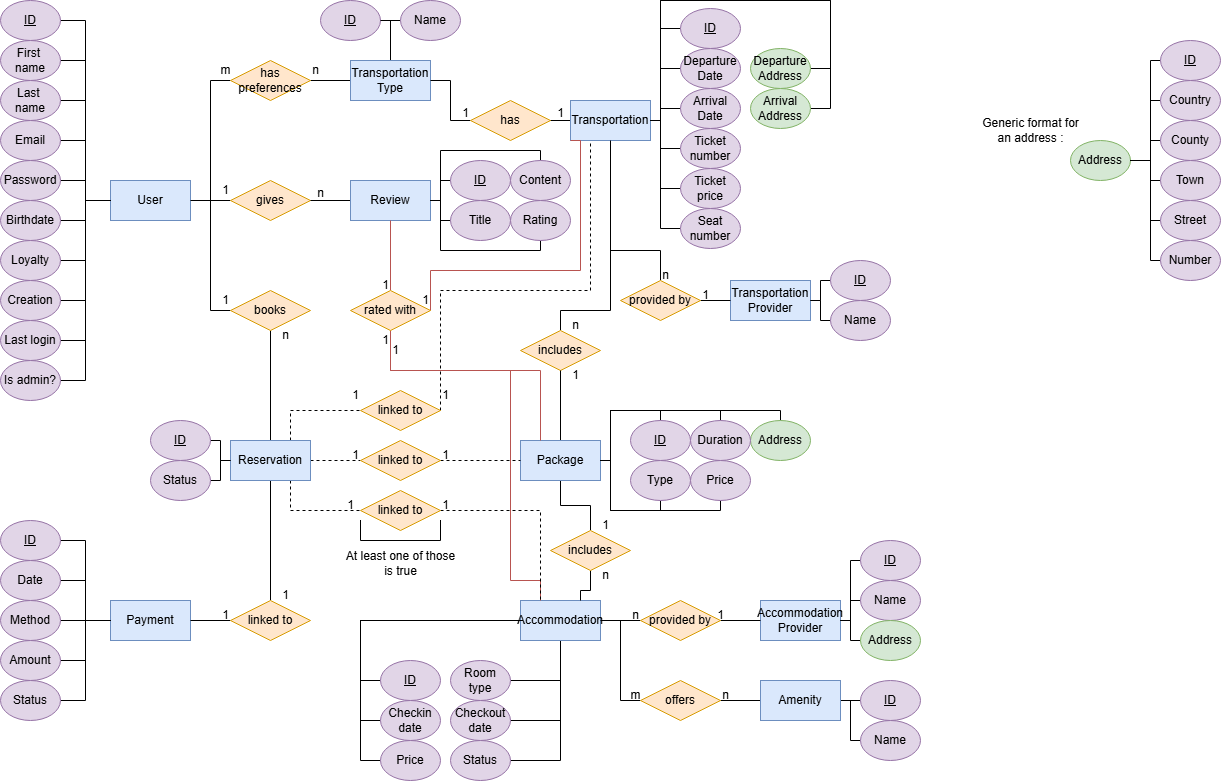
\includegraphics[width=450pt]{diag.png}
\newpage

\subsection{Database Designer View}
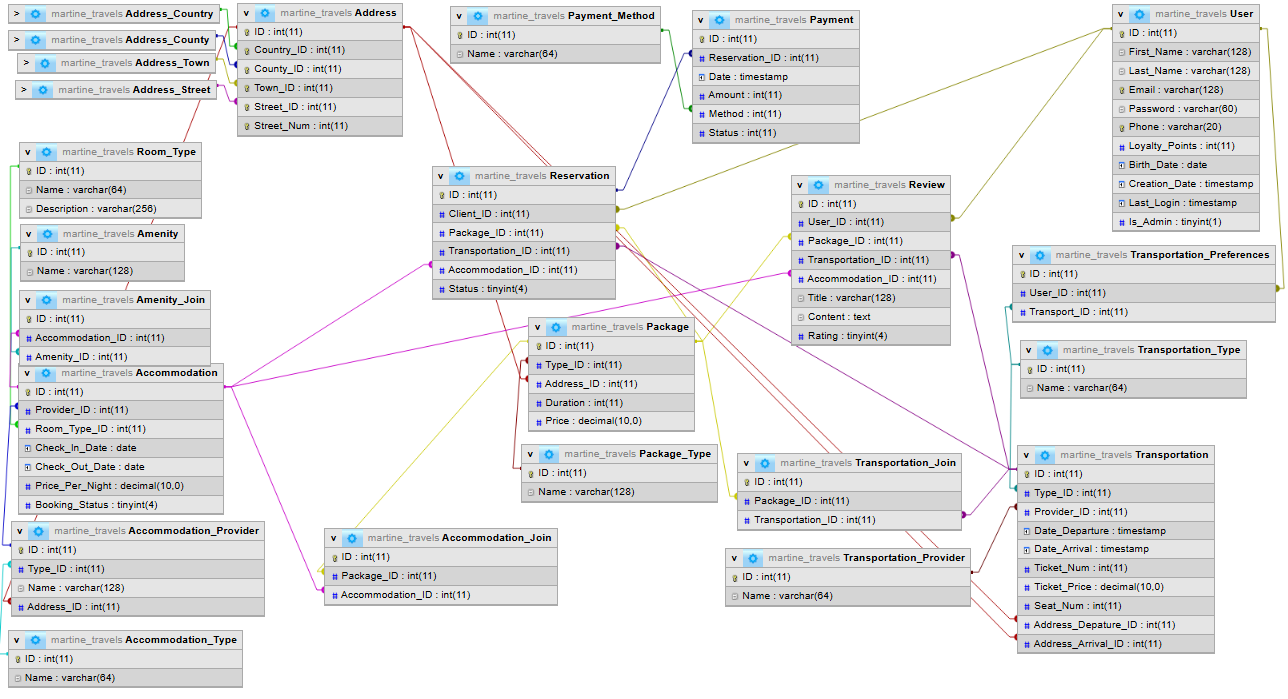
\includegraphics[scale=0.7,angle=90]{diag_2.png}

%-----------------------------------------------
\section{Front \& Back-end Design}
\paragraph{} 
Another important point of this work was to design and program a simple web interface in order to do at least "Login \& User Authentication", "Client Management", "Travel Package Management" and "Reservation System" pages. The latter are all explained down below.

\paragraph{}
The home page (\textit{a.k.a the homepage}) is \verb|site/index.php|. Also in order to offer a wonderful browsing experience to the user on our website, we decided to use CSS Styles to make the website more enjoyable. These can be found under \verb|site/css/|.

\subsection{Login \& User Authentication}
\paragraph{}
A user can sign into their account using the corresponding button within the header bar (\textit{which redirects them to main form of} \verb|site/signin.php|). If one does not have an account they can create one by \textit{signing up}. Then all required information are asked via a form. When trying to submit the latter, verification for data format coherence is performed by looking for regular expressions. For instance we make sure that a password is at least 8 characters long and contains at least one number, upper and lowercase letter. Also we make sure that an email address is only used once (\textit{i.e two users cannot have the same email address}). Yet we do not verify if it truly exists. Also for security purposes passwords are not directly saved into the database but rather a hash string ; we indeed use the \verb|PASSWORD_BCRYPT| to encrypt it.

\paragraph{}
When the user has been successfully log into their account they are either sent to the admin page if they happen to be one, or are redirected to their account page. Moreover the header bar updates itself and allows the user to log out and modify their settings.

\subsection{Administrator Access}
\subsubsection{Overview}

\paragraph{}
At the very beginning, we wanted to make an admin page such that every single table could be modified, be it adding a new record, updating lines with the right datatype, or deleting records. Very soon we discovered that this was not going to be possible for there is quite a number of tables, all of which are joined together. This led to chunks of duplicated code which could not be broken down into \verb|PHP| functions ; this was indeed due to the fact that almost every attribute had a different name whence unalike \verb|SQL| requests. 
\paragraph{}
Thereby we remade the entire page from scratch trying to write functions as it would ease our work. However this soon led to another issue. There are tables in which "secondary" IDs can reference others such as \verb|Package| or \verb|Address|. Thus a request will only return an ID, not the contents it is pointing onto. Hence we wrote a function which would display the latter (\textit{e.g we must show the first and last names of any user, and not just their ID}) and allow the administrator to easily modify any kind of record.
\paragraph{}
We've also decided to add an extra ID attribute for tables intervening in many-to-many relationships, which we will refer to as "\textit{Join Tables}". This enabled us to perform operations such as \textit{deleting or modifying} on any table without having to take care of every single case.
\paragraph{}
In order to prevent any staff member to enter invalid data or modify read-only attributes we set some rules down. First administrators are not allowed to directly modify any primary ID. Next forms will prevent anyone from sending data that is either invalid or in the wrong format/datatype (\textit{e.g text, timestamp, integer, \ldots}). Nevertheless there is no constraint on dates validity and coherence since scheduling is quite the task.
\paragraph{}
Finally there is a "\textit{super-admin}" which can be logged into using the following credentials:\\\verb|admin@gmail.com, admin|. By the way the reader must keep in mind that the password was so trivial to make testing easier, and to \textbf{never} use such weak passwords for any user with higher permissions. Moreover only an administrator can grant a user admin rights. 

\subsubsection{Code explanation}
\paragraph{}
Only administrators can enter the \verb|site/admin/admin.php| page. When one first arrive on that page they are asked to choose a table to modify. This can be done by clicking on the corresponding link. Then they are redirected to a page which displays all records from a table. This is because of a \verb|PHP| page of which two arguments are passed: the name of the table and the action to perform. The first one is used in \verb|DisplayTableData| which as its name suggests, displays the table. Then the second one is used in \verb|DisplayForm| which allows the admin to modify a record and checks for data format coherence.

\subsection{Reservation System}
\paragraph{}
Any client can choose to make a reservation (\textit{in their Account page}) whether pre made or personalized. The first one is the easiest as every information has already been entered by a staff member. The second one is trickier because everything must be done by the user and currently there is not enough data in the database to make a whole batch of different new packages.
\paragraph{}
The page \verb|site/add_reservation.php| asks for all those information and displays dynamically buttons and possible choices (\textit{according to the previous ones}) using JavaScript. This is done through another \verb|PHP| file which queries data from the database then creates a Json file from it. Next the latter is recovered and processed by a script which displays the new options.
\paragraph{}
At the end when all required data has been acquired a button labeled "Next" enables the user to finalize the reservation. Finally they can pay it by going on the "Payment" page.

\subsection{Other features}
\subsubsection{Inactive users deletion}
\paragraph{}
We have added a small scheduled event (\textit{every five minutes}) which looks for users who have not used the website in two years, then deletes the latter.

\subsubsection{Payment page}
\paragraph{}
When at a least one reservation has been made the client may choose to pay one with any of the supported payment methods. When those choices have been made a simple click on the button labeled "Pay" triggers the process.
\paragraph{}
In real life an other organization such as a bank takes care of money-related troubles ; our website must not store bank details as those are sensitive data. Indeed we should only receive a confirmation of the bank (\textit{or accommodation/transportation provider if using cash}) to mark the payment as completed. Thus we decided to simulate all these steps by a "pay" button.
\paragraph{}
When it has been done, another button to download the receipt appears. Also because we do not verify for dates coherence, the corresponding reservation is directly marked as "completed" instead of "pending".

\subsubsection{Reviews}
\paragraph{}
When a travel is marked as "completed", it appears on the home page and users are allowed to leave a review. However there isn't yet any code to display reviews.

%-----------------------------------------------
\section{Organization}
\paragraph{} 
In order to successfully complete our project and to be more efficient we adopted a simple rule: we made sure that everyone could work on the same file while being at home and without relying on a single person.

\subsection{Version Control System}
\paragraph{}
Using a version control system such as \textit{Git} was quite useful in our project as it enabled us to track and manage changes to the source code easily. It also allowed us to keep backups of the codebase in case something bad happened (\textit{e.g data corruption or loss, hardware malfunction}) or in case we wanted to try out new features without the fear of breaking something. Besides it made collaboration easier by allowing every member of the group to work on different aspects simultaneously.
\paragraph{}
We chose to host our code base on \textit{GitHub} as it is free and easier to set up in \textit{PhpStorm}. To access our project repository go \href{https://github.com/TheRefraction/Martine-travels}{here}.

\subsection{Connection to the Database}
\paragraph{}
The connection to the database has also been an important problem. Working separately on the database could indeed yield some interesting results to say the least. That is especially true when testing the front-end part ; one might have had a newer database model while another might not and thus would have had to update it (\textit{all records would have been lost}) to test the website. Therefore we chose to host the database on an UNIX Apache server run from a personal Raspberry PI card.
\paragraph{}
This solved a huge issue as now everyone could work on the project when they wanted to. Yet that simple action led to two sub-issues:
\subparagraph{Security}
We opened a port in our firewall to grant us a remote access to both the PhpMyAdmin page and the database. Yet anyone could also go through that port to steal information which is a great flaw. Thus, we first tried to enable SSL encryption, still it was too difficult to set up. So we set rules down in order to lower permissions for remote access. Moreover "suspicious" requests are denied by the Internet box. All in all this is okay for such a small project however keep in mind that those layers of security are not enough by today's standards.
\subparagraph{Static IP Address}
Another problem laid in the fact that we did not own a website domain, nor a \textbf{static} address as it cost money. Thus we had to use the IP address of the card every single time. Moreover most of the time an IP address will change about every two weeks. Thus someone had to monitor the latter and change it in \verb|connection.php| so as to ensure the connection to the database. 
\paragraph{}
For more information on how to connect to the database, please see Appendix \ref{DB_Connect}

%-----------------------------------------------
\newpage
\section{Conclusion}
\paragraph{}
In conclusion, this project showed us how databases can be used in daily life operations. We have also realized the significance of designing a thorough and normalized database structure ; indeed it must comprehensive by anyone who reads it and must limit redundancies. 

\paragraph{}
Moreover this subject is a tangible and realistic situation in which anyone can imagine themselves. As future engineers it is our job to ensure that the whole system works, thus we have a huge impact on the company's success. Also this work taught us to work and collaborate together, to express different ideas, compare opinions.

\paragraph{Difficulties}
We have faced four majors difficulties during this project. First of all in our view, the bill of specifications was sometimes too long or complicated. There were indeed too many entities and cases to manage at once, especially with transportation and accommodation providers. Secondly so as to implement some features (\textit{e.g the administrator page}), we had to read a big part of the \verb|PHP| and Javascript documentation, for which we spent a lot of time whereas we could have used it to enhance some features or add more things. Another big issue we have had is using XAMPP as it was (\textit{and still is}) a unstable piece of software. We've had indeed multiple occasions where we've had to uninstall and then reinstall XAMPP from the system, and it still would not work properly. Thus, the importance of using a mini-server on Linux. Moreover we preferred to use \verb|PHP| as a standalone software and configure the \verb|php.ini| file which took quite some time.
Finally, we think it may be better to have more students per group as there are many things to do. Despite it we realize that the more people in a group the more chaotic it can be. 

\paragraph{Suggestions}
Finally we have several things that we could have done to enhance the current codebase/database. After multiple tests, we think that splitting clients and staff member (\textit{e.g administrators}) into two tables might have been a good idea, for an admin should not be able to book a package and then mark the latter as "paid" manually (\textit{as of now an admin does not directly have access to the customers' homepage}). Next we could have stored images for travel packages in the database. Yet we did not have enough to add this feature through the back and front-end, and to make it so the database stays normalized. Finally we could have added a system to display reviews for a package.

%-----------------------------------------------
\newpage
\appendix
\section{Software used}

\begin{itemize}
	\item MariaDB 
	\begin{itemize}
		\item \underline{Server}: Localhost via UNIX socket
		\item \underline{Server connection}: SSL not set up
		\item \underline{Server version}: 10.11.8-MariaDB-0ubuntu0.24.04.1 - Ubuntu 24.04
		\item \underline{Protocol version}: 10
		\item \underline{Server character set}: UTF-8 Unicode (utf8mb4)
	\end{itemize}
	\item Apache/2.4.58 (Ubuntu)
	\begin{itemize}
		\item \underline{Database client version}: libmysql - mysqlnd 8.3.6
	\end{itemize}
	\item PHP 8.3.6 
	\begin{itemize}
		\item mysqli
		\item curl
		\item mbstring
		\item sodium
	\end{itemize}
	\item phpMyAdmin 5.2.1deb3
	\item PhpStorm 2024
\end{itemize}

\section{How to connect to the database?} \label{DB_Connect}
\paragraph{}
As of \today, the IP address of the server is \verb|90.100.91.219|. Also the server will be unplugged on December 1, 2024 at noon. Therefore you may try to access it remotely. However if you may prefer to upload the database on your localhost, there are some variables that need to be updated.
\paragraph{}
First start your Apache Server and import \verb|martine_travels.sql| into your PhpMyAdmin. Then open the file \verb|site/connection.php| and change its content to (\textit{assuming there is a user } \verb|root| \textit{with no password}):

\begin{verbatim}
<?php
function get_dbhandle(): PDO
{
	$host = "localhost";
	$dbname = "martine_travels";
	$dbuser = "root";
	$dbpasswd = "";
	return new PDO("mysql:host=$host;dbname=$dbname", $dbuser, $dbpasswd);
}
?>
\end{verbatim}

\end{document}
